\chapter{Results}
\label{chp:results}



With scikit-learn was a program created in python that reads through the dataset and puts the \gls{dns} calls in to an ndarray, which is a N-dimensional array. This is to easier use to right values for the machine learning model. The program also cleans up the dataset by removing some of the fields, which for this project seemed unnecessary. I created multiple scripts for taking out different sections of the dataset, to see if there would be any difference. The code for the parser program is in \ref{chp:parserprogram}

The main program read through a \texttt{csv} file, the dataset, and put each line as an array in a ndarray. N-dimensional array is a numpy class which is beneficial to use with scikit-learn. Further the ndarray was preprocessed to scale everything to a similar level. This level is set by calculating the mean and standard deviation of the ndarray. 

The different classifiers are initiated with parameters that is changed to see what best fit the data. As the data is unlabeled, it is impossible to know how many of the observations are a part of a \gls{dns} tunnel if there is any. The classifiers must not have any inputs, but it will help making them more precise. In this project the contamination level, which is the level of data which is viewed as incorrect, was first calculated as the percentage of observations which was over average as a base. The value has been change up and down, but kept in the same area. 

To be able to show the solutions and really understand what the machine learning model did, all of the experiments used two dimensions. The dimensions change between $downlink, uplink, duration, downlink/duration$ and $uplink/duration$. The values was not marked with any type, but based on network theory is duration set to the of length of conversation in seconds. The uplink and downlink is  the number of bytes transferred up to the server or downloaded from the server, respectively.

Since it was no known \gls{dns} tunnels in the dataset, it is impossible to use precision, recall or the $F_1$ measure as results. The precision and recall measurements are defined in algorithm \ref{recallPrecision}. The $F_1$ measurement was defined van Rijsbergen \cite{manevitz2002one} as a way of combining precision and recall. The formula is in algorithm \ref{f1}. As seen from the definitions without the knowledge of tunnels in the dataset will there not be a way of measuring the correctness of the machine learning algorithms.

\begin{algorithm}

$$ recall = \frac{Number of items of a category identified}{Number of items in the category in the dataset} $$

$$ precision = \frac{Number of items of a category identified}{Number of items classified to the category} $$

\caption{Recall and precision definitions}
\label{recallPrecision}
\end{algorithm}

\begin{algorithm}
\caption{$F_1$ measure}
\label{f1}
$$ F_1(R,P) = \frac{2RP}{R+P} $$
\end{algorithm}


\begin{figure}[hbp]
\centering
	\begin{subfigure}[b]{0.4\textwidth}
		\centering
		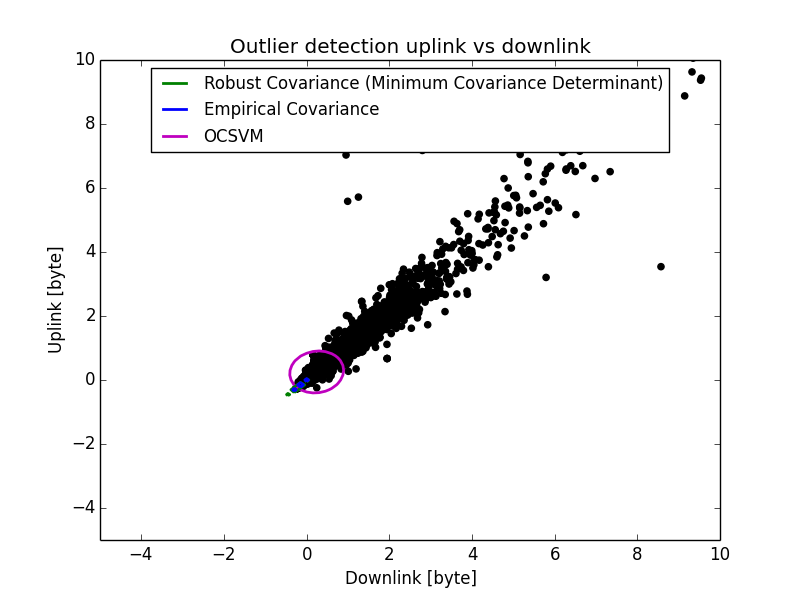
\includegraphics[scale=0.28]{figs/scaleUpVSDown.png}
        \caption{Scaled data}
        \label{fig:scaledUpDown}
	\end{subfigure}
	\begin{subfigure}[b]{0.4\textwidth}
		\centering
		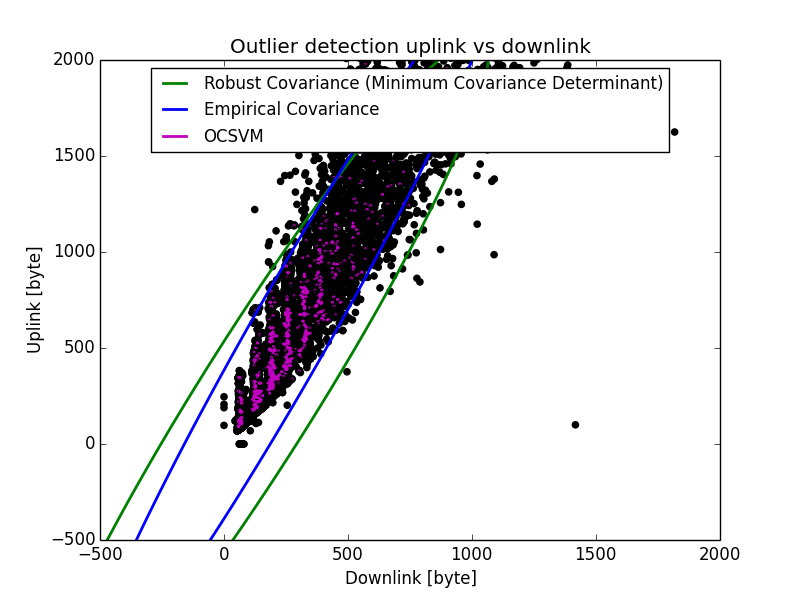
\includegraphics[scale=0.28]{figs/unscaledUpVSDown.png}
		\caption{Unscaled data}
		\label{fig:unscaledUpDown}
	\end{subfigure}
\caption{Difference between scaled and unscaled data}
\label{fig:scaledVSUnscaledUpDown}
\end{figure}


\section{Scaled data vs unscaled data}
As seen in \fref{fig:scaledVSUnscaledUpDown} the scaled and unscaled graphs bears the same characteristics. Most of the observations has almost the same value for uplink and downlink. 
The results were better for \gls{ocsvm} with scaled data, while the covariance calculations worked better with the unscaled. The unscaled data spreads so far out that it is hard to see all the data points, while the scaled data is more compact giving a better overview. The ellipses on the figures is the learned decision of the classifier model. Meaning that inside the ellipses is the area where an observation is considered normal. Since the \gls{ocsvm} is the main focus, scaled data was used for the rest of the experiments.

\section{Different axes}
Next up was looking which values would be best for the axes to represent the data. In \fref{fig:scaledVSUnscaledUpDown} the fields of the dataset used were \texttt{uplink} and \texttt{downlink}. This were the first thoughts of finding irregularities, as mentioned in chapter \ref{chp:dns_detection} this is a volume analysis comparing total volume from a user in one \gls{dns} session. \fref{fig:updurAndspeed} shows graphs where other fields of the data set were used as input for the model. In \fref{fig:scaledUpDur} the size of the uploaded data were compared to the time the session were used, this shows that there are a number of users in the same area which the model learn as the normal area, which in scale is around 0. The result were similar when changing uplink with downlink. There are users uploading and downloading lots of data in short time, this lead to the idea of introducing a new field to the dataset. Combining the discoveries from \fref{fig:scaledUpDown} and \fref{fig:scaledUpDur}, by seeing how much data where uploaded or downloaded during a session. This is depicted in \fref{fig:scaledUpDownDivDur}. In this graph it is possible to see that the observation is even more clustered. This seemed like a good representation. 


\begin{figure}
\centering
	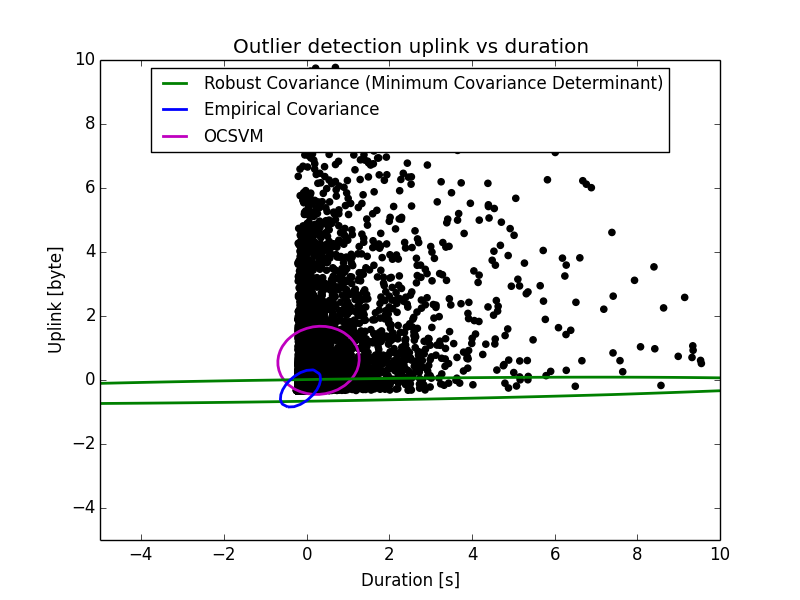
\includegraphics[scale=0.6]{figs/scaleUpVSDur.png}
	\caption{Uplink vs duration of session. }
	\label{fig:scaledUpDur}
\end{figure}


\begin{figure}
	\centering
	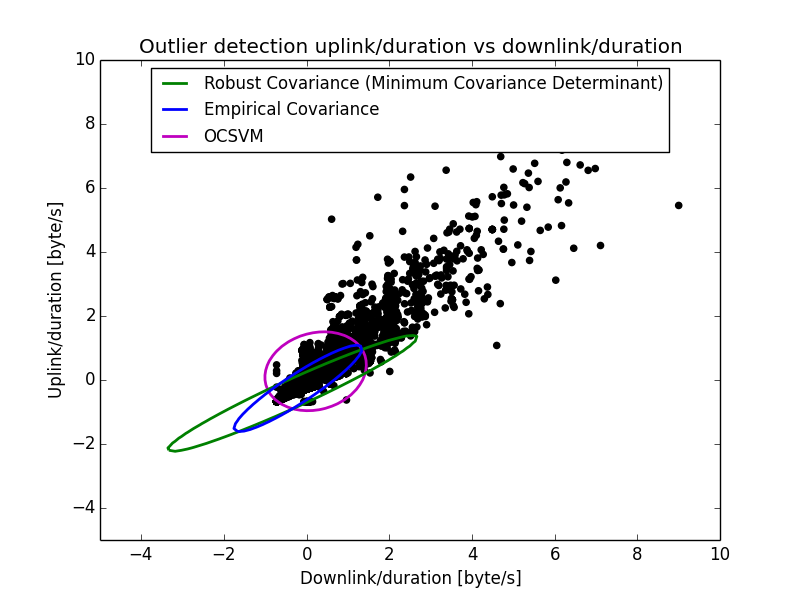
\includegraphics[scale=0.6]{figs/scaleUpDivDurVSDownDivDur.png}
	\caption{Average speed in each direction}
	\label{fig:scaledUpDownDivDur}
\end{figure}

\section{Different parameters}
The fields of the dataset is, as mentioned earlier, not the only variable when finding the best way for a model to fit to the dataset. The machine learning model has parameters that is given when instantiated. For \gls{ocsvm} is it possible to set what kind of kernel it should use and the number of training errors among others. \texttt{Kernel} is the function the model should use. The number of training errors, \texttt{nu} in scikit-learn, is the upper bound fraction of outliers in the training set, and the lower bound of training examples used as support vectors. For this project the kernels used where \texttt{rbf} and \texttt{linear} where rbf is the one used in the graphs so far. 
The nu was first set to $0.15$ which was calculated as the fraction of observations above average, this has been changed to see how it affect the learned decision. In $ $ $ $ do you see how changing nu is affecting the model. It is clear to see that in this dataset there are a low fraction of observations that does not fit the model. Using the linear kernel the model tries to find a linear line it can draw where all observations on one side is correct observations and on the other side is outliers. This is seen in $ $ $ $ $ $. It was worth a try, but it seems that rbf if the best kernel. 